\chapter{Обзор литературы} \label{chapt1}

\section{Современное состояние исследований оптических частотных гребенок в микрорезонаторах} \label{sect1_1}

Развитие фемтосекундных оптических частотных гребенок, отмеченных Нобелевской премией в 2005 г. \cite{Hall2006}, оказало огромное влияние на науку и технологии с момента их первоначального открытия в 2000 году. Помимо хорошо известных приложений в прецизионной частотной метрологии и для создания атомных часов \cite{Diddams2001,Udem2002,Ye2005,Diddams2004}, возможность эффективно управлять амплитудой и фазой точно определенных спектральных компонент открыло совершенно новые подходы для генерации аттосекундных импульсов \cite{Jones2000,Telle1999} спектроскопии \cite{Stowe2008,Diddams2007,Ideguchi2013,Holzwarth2000}, обработки оптических сигналов и радиофотоники \cite{Gao2006,Torres2014} и также для многих других важных практических приложений \cite{Newbury2011,Steinmetz2008,Fortier2011}. Открытые в лаборатории профессора Киппенберга в 2007 году керровские оптические частотные гребенки в оптических микрорезонаторах (микротороидах) из плавленого кварца \cite{DelHaye2007,Kippenberg2011} вызвали еще одну революцию в области метрологии. Керровские гребенки позволяют достичь уровня миниатюризации и энергоэффективности, труднодостижимого для гребенок, полученных с помощью фемтосекундных лазеров в режиме синхронизации мод, что в свою очередь позволяет существенно уменьшить размеры генераторов гребенок и создавать их на одном чипе, что в настоящее время исследуется во множестве лабораторий, в частности, в США. Число статей, публикуемых в год по этой тематике, достигает сейчас почти 100 и продолжает расти с каждым годом.


Возможность синтезировать частотные гребенки непосредственно на чипе открывает путь к полностью интегрированным генераторам оптических гребенок, которые могут существенно упростить процессы измерения и синтеза частоты, и, тем самым, выйти на коммерческий рынок. Основными преимуществами частотных гребенок из микрорезонаторов являются их компактность, высокая мощность, приходящаяся на каждую компоненту гребенки, и возможность получения частот повторения в диапазоне 10-1000 ГГц, важном для многих приложений, включая телекоммуникации высокой пропускной способности \cite{Pfeifle2014}, астрофизику \cite{Glenday2015}, синтез частот \cite{Ferdous2011}, радиофотонику и генерацию микроволн \cite{Xue2016,Savchenkov2008}. Оптическая частотная гребёнка может быть использована как высокостабильный калибровочный репер для прецизионной спектроскопии, как источник спектрально чистого СВЧ сигнала, а также для генерации фемтосекундных оптических импульсов – генераторы гребенки могут обеспечивать короткие периодические оптические импульсы (солитоны длительностью ~300 фс в кристаллических и ~20 фс в интегральных) с очень малым временным джиттером. Параметрический характер усиления обеспечивает широкополосность процесса в полосе, достигающей октавы. Подобный спектр гребенки может связывать оптический диапазон с микроволновым и наоборот. Кроме того, ширина полосы усиления ограничена только окном прозрачности материала микрорезонатора, что позволяет генерировать гребенки как в УФ, так и среднем ИК диапазонах.


В последние годы наблюдается быстрый и существенный прогресс в области микрорезонаторных частотных гребенок. Гребенки были продемонстрированы в различных структурах, в том числе в кристаллических резонаторах из различных фторидов \cite{Savchenkov2008,Grudinin2012,Jost2015,Liang2011,DelHaye2011,Chembo2010,Grudinin2009}, в интегральных микрорезонаторах из нитрида кремния (SiN) [30-33], в планарных системах, изготовленных из стекла Hydex [34,35], а также во многих других диэлектрических материалах [36,37]. Такие гребенки были использованы для обоснования различных концептуальных приложений, в том числе, демонстрации оптических атомных часов, синтеза оптических сигналов, демонстрации подсчета периодов световой волны, а также когерентной связи с терабитной скоростью. Недавние эксперименты швейцарской группы продемонстрировали передачу данных на расстояние 300 км с терабитной скоростью при квадратурной амплитудной модуляции [19].


Кроме того, с момента открытия был проведен численный анализ и достигнуто понимание богатой нелинейной динамики процесса формирования гребенок; объяснены механизмы появления шумов в керровских гребенках [38], а также были определены состояния, отвечающие низким уровням шума. Следует отметить, что в отличие от частотных гребенок, получаемых при синхронизации мод лазера, произвольные микрорезонаторные частотные гребенки не представляют собой сверхкороткие импульсы во временном представлении из-за произвольных фазовых соотношений между отдельными спектральными линиями, появляющимися в процессе формирования гребенки. Решить эту проблему и получить малошумные, когерентные частотные гребенки с гладким спектральным профилем можно путем генерации диссипативных керровских солитонов. Для этого был предложен и продемонстрирован новый метод генерации микрорезонаторных оптических гребенок на основе временных солитонов в оптических микрорезонаторах [39]. Предложенный метод основан на плавном изменении частоты накачки, приводящем к формированию временных солитонов. Этот результат стал большим прорывом в области, поскольку позволил генерировать когерентные и широкополосные оптические гребенки, которые могут быть достигнуты детерминировано и могут быть смоделированы с помощью уравнения Луджиато-Лефевра. Также эта работа показала возможность генерации фемтосекундных когерентных периодических оптических импульсов с малым джиттером. Недавно, с помощью этого метода солитоны были получены в кварцевых микрорезонаторах, изготавливаемых методом фотолитографии [41]. Позже были описаны механизмы, препятствующие образованию солитонов в микрорезонаторах, и методы их преодоления [42]. В недавней работе показали формирование и распространение солитона и генерацию гребенки в 2/3 октавы в микрорезонаторе, интегрированном на чип [43].  В целом, в последнее время появилось множество работ, посвященных генерации и свойствам солитонов в микрорезонаторах или, что тоже самое, но в частотном представлении, солитонным (когерентным) керровским оптическим частотным гребенкам [44-54].


В то же время в последние несколько лет было предложено несколько перспективных методов, позволяющих обойтись без значительной перестройки частоты лазера накачки: один из них базируется на использовании фазомодулированной накачки [55,56], а второй – на тепловых эффектах [57,58], в том числе и с использованием дополнительного нагревательного элемента [58]. При нагреве микрорезонатора происходит сдвиг резонансных частот микрорезонатора относительно частоты накачки, что в какой-то мере эквивалентно ранее описанному процессу перестройки частоты лазера накачки. Также было показана возможность получения односолитонного режима, важного для практических применений. Это осуществлялось либо контролируемым нагревом и охлаждением нагревательного элемента, либо обратной медленной перестройкой частоты лазера накачки [59]. Также недавно был продемонстрирован метод генерации солитонов с помощью интегрированных PIN-структур, позволяющих контролировать время жизни свободных носителей заряда [60].


Одной из приоритетных задач в области микрорезонаторных частотных гребенок является расширение спектрального покрытия существующих керровских гребенок. Эта задача представляет широкий интерес и, например, является приоритетным направлением в грантовой программе SCOUT (Spectral Combs from UV to THz – Спектральные гребенки от ультрафиолета до терагерцового диапазона), запущенной в США агентством DARPA [61].


Перспективным направлением исследований является генерация керровских частотных в среднем ИК диапазоне. Этот диапазон интересен тем, что в нем находятся колебательные уровни многих молекул, из-за чего его называют диапазоном “молекулярной дактилоскопии” [9]. К таким молекулам относятся углеводороды, вещества, важные для экологии, токсичные химикаты. В настоящее время средний ИК изучается в основном с помощью инфракрасных-Фурье спектрометров (ИКФС) [62]. Оптические гребенки в среднем ИК могут представлять собой очень интересное технологическое решение для молекулярной дактилоскопии, а компактный источник частотной гребенки в среднем ИК может обеспечить значительный потенциал для расширения возможностей и областей применения среднего ИК диапазона. С одной стороны, он может быть использован в качестве яркого источника для Фурье-спектрометра. Более интересной является перспектива использования таких компактных устройств для спектроскопии с использованием двух гребенок (назовем для краткости двухгребеночная спектроскопия) [63-66], когда сбиваются два источника гребенок в среднем ИК с различными частотами повторения, и генерируется сигнал биений на фотодетекторе в форме гребенки, но уже в радио диапазоне частот, что может быть использовано для восстановления профилей поглощения веществ в быстром, компактном устройстве без подвижных механических частей.


Тем не менее, технология генерации керровских гребенок в среднем ИК остается сравнительно слаборазвитой и количество публикаций, посвященных этой проблеме, сравнительно мало [67-71]. В частности, в экспериментах, проведенных в EPFL при использовании параметрического лазера непрерывного излучения в качестве накачки, проф. Киппенберг в сотрудничестве с Т. Хэншем и Н. Пике показали возможность генерации оптических гребенок в среднем ИК на длине волны 2.5 мкм [68]. Генерация в среднем ИК также была продемонстрирована в структурах из нитрида кремния [60, 69, 70]. Также генерация гребенки со спектральной шириной, превышающей половину октавы, была продемонстрирована в микрорезонаторах из CaF2 и MgF2 при накачке квантово-каскадным лазером [71]. В основном же для генерации гребенок в среднем ИК успешно применялись такие подходы, как параметрическая генерация или генерация разностной частоты [72-75], однако ширина полосы и величина мощности, приходящейся на каждую компоненту гребенки, а также степень когерентности остаются ограниченными так же, как и габариты экспериментальной установки. Поэтому создание эффективного компактного генератора когерентных керровских гребенок в среднем ИК является очень важной задачей. В качестве материала, пригодного для генерации частотных гребенок в среднем ИК, в последнее время широко обсуждается фторид бария [76-77] и другие фториды [78-79].


Еще одним чрезвычайно важным направлением исследований является возможность генерации когерентных гребенок в режиме нормальной дисперсии [80], то есть в видимом и ближнем ИК диапазоне длин волн, т.к. материальная дисперсия большинства исследуемых материалов в этих диапазонах является нормальной. Что касается видимого диапазона [81, 82], следует отметить, что керровские частотные гребенки с большим межмодовым расстоянием могут, в частности, использоваться для астрофизических измерений [83, 84] и приложений рамановской спектральной визуализации. Также возможно применением керровских гребенок в видимом диапазоне и ближнем ИК для двухгребеночной спектроскопии [85]. Видимый диапазон привлекателен еще и тем, что в нем возможна визуализация биологических веществ из-за наличия в нем окна спектра пропускания воды, и он также характеризуется большими сечениями комбинационного рассеяния. Отметим, что в основном до настоящего времени для генерации частотных гребенок в видимом диапазоне использовалось совместное действие квадратичной и кубичной нелинейностей [81, 82].


Из-за наличия пиков поглощения в УФ многие диэлектрические материалы имеют нормальную дисперсию групповых скоростей (ДГС) в видимом диапазоне и ближнем ИК, что препятствует генерации светлых солитонов. Экспериментально узкие керровские частотные гребенки при нормальной ДГС были получены в кристаллических микрорезонаторах [86-89] и микрокольцах на чипе [90]. Также было теоретически и экспериментально продемонстрировано существование темных временных солитонов [44, 91-94]. В частности, в ряде работ существование темных солитонов было связано с наличием волн переключения между двумя плосковолновыми состояниями [93-94]. Однако на сегодняшний день полное понимание динамики этого процесса, в том числе механизмов, обеспечивающих генерацию керровских частотных гребенок с малым шумом в режиме нормальной дисперсии, отсутствует.


Недавно был численно показан новый класс солито-подобных импульсов, под названием “платиконы” ("platicons"), которые существуют в нормальном режиме дисперсии групповой скорости [92]. Было показано, что, меняя частоту накачки, можно управлять длительностью подобных импульсов. С точки зрения преобразования энергии накачки в энергию генерируемых импульсов генерация широких платиконов оказалась более эффективной, чем генерация обычных светлых солитонов. Также было обнаружено, что для нормальной дисперсии боковые линии гребенки, ближайшие к накачке, существенно более интенсивны, чем при аномальной дисперсии, что очень важно для создания радиофотонных генераторов СВЧ на основе гребенок. Описанная выше генерация платиконов была описана для систем с дефектом закона дисперсии, вызванным, например, взаимодействием мод различных семейств [42, 95] или эффектом затягивания частоты излучения лазера накачки на моду высокодобротного микрорезонатора. Было показано, что в системе с двумя связанными микрорезонаторами этим взаимодействием можно управлять [96]. Также, недавно было показано, что мягкое возбуждение платиконов возможно и без модификации закона дисперсии при двухчастотной накачке или при достаточно сильной амплитудной модуляции накачки с разницей частот кратной области свободной дисперсии резонатора (ОСД)[97]. Применимость этой методики подтверждается тем, что ранее при ее помощи теоретически [98] и экспериментально [99] было продемонстрирована генерация керровских частотных гребенок в режиме аномальной дисперсии. Также недавно была продемонстрирована генерация частотной гребенки в оптоволокне с нормальной дисперсией при двухчастотной накачке [100].


Еще одним актуальным направлением исследований в области микрорезонаторных частотных гребенок является разработка методов увеличения их ширины и когерентности. Одним из исследуемых в последнее время способов является взаимодействие временных солитонов и дисперсионных волн (иногда по аналогии называемых, индуцированным  солитонами черенковским излучением) [43, 101-107]. При накачке микрорезонатора в области аномальной дисперсии возможна генерация солитона. Если его длительность достаточно мала, то его спектр распространяется в область нормальной дисперсии и солитон может генерировать дисперсионную волну – пик излучения вблизи точки нулевой дисперсии. Формирование дисперсионной волны в присутствии солитона может способствовать уширению полосы генерации гребенки в область нормальной дисперсии без потери когерентности. Таким способом была экспериментально продемонстрирована генерация гребенки в 2/3 октавы в микрорезонаторе, интегрированном на чип при накачке на длине волны 1.55 мкм (рис. 11) [43].


Для генерации и реализации эффективного взаимодействия солитонов и дисперсионных волн должны выполняться определенные дисперсионные соотношения, поэтому разрабатывается множество методов получения оптимальной дисперсии (dispersion engineering). Дисперсия кристаллического резонатора может быть специально задана [28, 108-113], например, с помощью микроструктурирования его формы [112, 113]. В частности, было продемонстрировано, что эффективно изменять дисперсию можно путем прецизионного формирования микрометрических выступов [112]. Также специально рассчитанная форма поперечного сечения микрорезонатора может обеспечить аномальную дисперсию в диапазоне, превышающем октаву [113]. 

TODO: обзор ТГц гребенок, окатава + оптический синтезатор частот

Большой интерес привлекает возможность использования эффектов рамановского и бриллюэновского рассеяния для генерации частотных гребенок и контроля их свойств. Например, активно исследуется влияние рамановского рассеяния на генерацию и свойства диссипативных солитонов в оптических микрорезонаторах (например, эффект сдвига спектрально максимума солитона, Raman induced soliton self-frequency shift) [114-119]. Также в нескольких недавних работах [120-121] исследовалась возможность генерации оптической частотной гребенки в полосе рамановского рассеяния в области нормальной дисперсии групповой скорости, где обычные методы, как было уже сказано, работают плохо. В работе [120] экспериментально была продемонстрирована генерация оптической частотной гребенки в кристаллическом резонаторе из MgF2 при накачке 1064 нм в присутствии интенсивного спектрального максимума, вызванного вынужденным комбинационным рассеянием. Это было интерпретировано авторами как совместное воздействие эффектов Рамана и Керра (Kerr-Raman interaction). Этот результат открывает новый путь к пути к генерации оптических частотных гребенок в области нормальной дисперсии групповой скорости. Однако теоретические выводы авторов основанные на численном решении уравнения Луджиато-Лефевра значительно расходятся с экспериментальными результатами и не позволяют в полной мере проанализировать процесс генерации гребенки и ее когерентные свойства.


Другой актуальной задачей является генерация и изучение свойств частотных гребенок в средах, обладающих как кубической, так и квадратичной нелинейностями [122]. Такими средами являются, например, кристаллы ниобата лития и танталата лития. Также, как было показано недавно, квадратично-нелинейные эффекты могут проявляться и в микрорезонаторах, изготовленных из центросимметричных материалов (кремний, нитрид кремния) из-за механических напряжений и поверхностных эффектов [81]. Наличие квадратичной нелинейности позволяет наблюдать нелинейные эффекты как на первой, так и на второй гармониках накачки, что может привести к чрезвычайному уширению керровской частотной гребенки, генерируемой в такой среде, и переносу ее в другой диапазон. Ширина полосы такой гребенки может превысить октаву. Таким образом, например, были получены частотные гребенки в видимом диапазоне в микрорезонаторах из нитрида кремния [81] и нитрида алюминия [82]. Совместное действие квадратичной и кубичной нелинейностей могут также существенно изменить свойства диссипативных солитонов.


В недавних работах было показано, что возможна прямая генерация частотной гребенки в кристалле периодически поляризованного ниобата лития, помещенного во внешний резонатор [123]. Использование микрорезонаторов позволит увеличить добротность, что снизит порог по мощности накачки. Материалы с ненулевой квадратичной нелинейностью, в отличие от центрально-симметричных, в которых генерация керровских гребенок изучена намного более полно, обладают большим разнообразием эффектов, которые позволяют управлять процессом генерации гребенки и ее параметрами. Так кристаллы ниобата лития являются двулучепреломляющими, обладают электрооптическим, собственным пьезоэлектрическим, пироэлектрическим эффектами, а также фотоупругим эффектом. Отдельной важной задачей является вопрос достижения условия фазового синхронизма при трехволновом взаимодействии в анизотропной среде. Стандартной методикой на данный момент является использование периодически поляризованных образцов, структура поляризации которых позволяет достичь квазисинхронизма. Вопрос об оптимальной структуре периодической поляризации, которая бы обеспечила оптимальную перекачку энергии, остается открытым. Отметим, что в средах с квадратичной нелинейностью условия фазового синхронизма играют такую же роль для генерации частотных гребенок, что и знак дисперсии в кубично-нелинейных кристаллах.
Важной задачей является разработка новых устройств для генерации микрорезонаторных гребенок на едином чипе. Одной из конструкций может быть микрорезонатор, связанный через затухающее поле, например, с экситонами в квантовых ямах с электрической или оптической накачкой. Эта система может работать в режимах сильной связи, когда образуются поляритоны [124]. Поляритоны существуют в относительно узком спектральном диапазоне вблизи экситонного резонанса, где накачка и сильная поляритонная нелинейность включают процесс параметрического преобразования, который запускает генерацию широкой гребенки уже в фотонном (неполяритонном) режиме. Идея связи микрорезонатора с усилителем недавно была проверена в эксперименте, в котором микрорезонатор был помещен в виток волоконного усилителя (EDFA) и была получена гребенка [125]. Недавняя теоретическая работа по поляритонным гребенкам рассматривала модель узкой резонансной полосы частот, где могут существовать лишь несколько спектральных линий [126].


Рассмотрим более подробно основные достигнутые результаты по генерации оптических частотных гребенок и солитонов, их количественные характеристики и основные продемонстрированные применения.

Первое экспериментальное наблюдение оптического гребенок в микрорезонаторах было продемонстрировано в 2007 году в работе \cite{comb_nature_2007}. Использовался резонатор в форме тороида из плавленого кварца, размещенный на кремниевой подножке. Добротность резонатора составила $Q=10^8$. Связь с резонатором осуществлялась с помощью растянутого оптоволокна. Накачка проводилась непрерывным лазером на длине волны $1550$ нм и мощностью $50$ мВт. Наблюдалась генерация боковых мод в сторону больших и меньших частот от накачки. За счет процессов четырехволнового взаимодействия гребенка расширялась. Для тороида диаметром $75$ мкм возбуждалось более 70 мод, почти равномерно покрывающих диапазон в $500$ нм. Для резонатора большего диаметра ($190$ мкм) наблюдалась гребенка шириной $380$ нм, содержащая 134 моды, с межмодовым интервалом $375$ ГГц. Был проведен эксперимент по проверке эквидистантности мод полученной гребенки путем сравнения ее с эталонной гребенкой, генерируемой импульсным лазером в нелинейном волокне (по Т. Хэншу). Равномерное распределение мод (эквидистантность) была подтверждена с высокой точностью. В работе проведено измерение дисперсии, она положительна, т.к. материальная дисперсия $\Delta\nu_{FSRmat}$ в плавленом кварце компенсирует отрицательную геометрическую дисперсию $\Delta\nu_{FSRgeom}$. Дисперсия групповой скорости $GVD$ в плавленом кварце положительная для длин волн больше $1.3$ мкм.

\begin{equation}
\Delta\nu_{FSR}=(\nu_{m+1}-\nu_m)-(\nu_m-\nu_{m-1}),
\end{equation}
\begin{equation}
\Delta\nu_{FSRgeom}\approx-0.41\frac{c}{2\pi nR}m^{-\frac{5}{3}},
\end{equation}
\begin{equation}
\Delta\nu_{FSRmat}\approx\frac{c^2\lambda^2}{4\pi^2n^3R^2}GVD,
\end{equation}
\begin{equation}
GVD=-\frac{\lambda}{c}\frac{\partial^2 n}{\partial \lambda^2},
\end{equation}
где $\nu_m$ - частота моды с номером $m$, $c$ - скорость света, $n$ - показатель преломления среды, $R$ - радиус резонатора, $\lambda$ - длина волны.

В работе \cite{octave_comb_2011} продемонстрирована генерация октавной гребенки. Этого удалось добиться за счет оптимизации дисперсии резонатора (путем численного моделирования его геометрии), увеличения его добротности и мощности лазера накачки. Экспериментальная установка состоит из диодного лазера, сигнал которого усиливается эрбидиевым волоконным усилителем (EDFA) до выходный мощности $2.5$ Вт. Связь с резонатором осуществляется через растянутое волокно. Из-за большой мощности накачки моды резонатора испытывают термический сдвиг, требуя большой перестройки лазера накачки (до $1$ ТГц), чтобы оставаться в резонансе с модами микрорезонатора. Гребенка наблюдается с помощью двух оптических спектроанализаторов. При накачке на частоте $1560$ нм в резонаторе наблюдается спектр гребенки, покрывающий одну октаву (рис. \ref{octave_comb_mlg}). Для резонатора диаметром $80$ мкм и добротностью $Q\approx2.7\times10^8$ межмодовое расстояние гребенки составляет $850$ ГГц. Измеренное значение ширины линии гребенки $\approx 70$ МГц. В работе продемонстрирована возможность перестройки лазера накачки более, чем на одну область свободной дисперсии (до $500$ ГГц) с сохранением генерации октавной гребенки, покрывающей диапазон $140-280$ ТГц.
\begin{figure}
  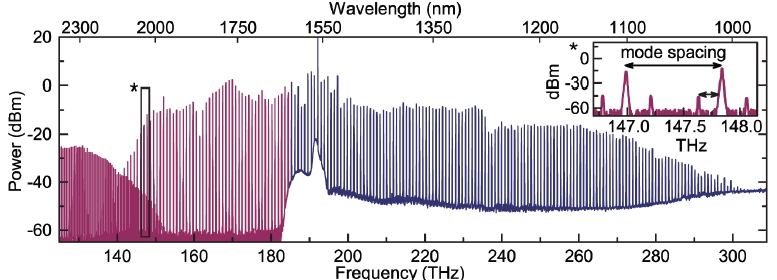
\includegraphics[]{octave_comb_mlg}
  \caption{Спектр октавной гребенки, полученной из тороидального резонатора из плавленого кварца диаметром $40$ мкм. Расстояние между линиями гребенки $850$ ГГц. Взято из \cite{octave_comb_2011}}
  \label{octave_comb_mlg}
\end{figure}


В работе \cite{MLG_nature_2012} экспериментально изучалась динамика генерации гребенок в двух различных резонаторах: $MgF_2$ (ширина резонанса $1$ МГц), и $Si_3N_4$ (200 МГц). Геометрии резонаторов изображены на рис. \ref{mgf2_si3N4_resonators}.

\begin{figure}
  \centering
  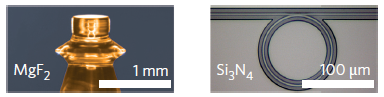
\includegraphics[]{mgf2_si3N4_resonators}
  \caption{Форма резонаторов для наблюдения оптических гребенок. Взято из \cite{MLG_nature_2012}}
  \label{mgf2_si3N4_resonators}
\end{figure}
Для генерации первых боковых мод и далее всей гребенки лазер накачки постоянной мощности изначально сильно отстроен в синюю область от резонансной моды. Далее отстройка накачки медленно уменьшается, так что все больше и больше света связывается с резонансом. В некоторой точке достигается параметрический порог и возникает первая пара боковых мод. Экспериментальный вид спектра гребенок для обоих резонаторов представлен на рис. \ref{universal_formation_mlg}. Рассматриваются 2 сценария развития гребенки: а) первые образовавшиеся боковые моды являются соседними к моде накачки резонатора; б) первые боковые моды образуются вдалеке (по номеру моды) от накачки. Используется разложение собственных мод невозбужденного резонатора $\omega_\mu=\omega_0+D_1\mu+\frac{1}{2}D_2\mu^2$, где $D_1$ соответствует ОСД резонатора, $D_2$ - разность двух соседних ОСД около центральной частоты $\omega_0$. Далее аналитически решается система связанных уравнений для двух боковых мод и моды накачки. Собственные значения этой системы дают условие на порог генерации боковых мод. Откуда можно получить выражение для минимального номера первично возбуждаемых мод $\mu_{th,min}=\sqrt{\frac{\kappa}{D_2}}$, где $\kappa$ обозначает суммарные потери в резонаторе и элементе связи.
\begin{figure}
  \centering
  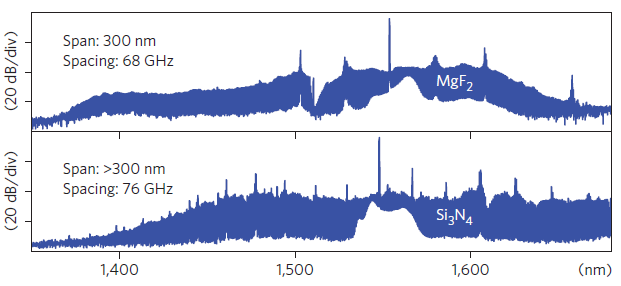
\includegraphics[]{universal_formation_mlg}
  \caption{Спектр наблюдаемых гребенок. Мощность накачки для $MgF_2$ - $500$ мВт; для $Si_3N_4$ - $3$ Вт. Взято из \cite{MLG_nature_2012}}
  \label{universal_formation_mlg}
\end{figure}

В работе \cite{Chembo_modal} приводится общее описание сферических микрорезонаторов с модами типа шепчущей галереи (МШГ), дается вывод системы связанных уравнений (спектральное представление), описывающих динамику каждой моды. Аналитически выводится значение пороговой мощности, необходимой для начала генерации гребенки $P_{th}=\frac{n_0^2 V_0}{2\hbar\omega_0 n_2 c Q_0}$, где $n_0$ - показатель преломления, $V_0$ - эффективный объем моды, $\omega_0$ - частота накачки, $Q_0$ - собственная добротность резонатора, $n_2$ - нелинейная часть показателя преломления. В статье проведено численное моделирование этой системы для $200$ мод.

Оптические гребенки наблюдались при разных геометриях резонаторов и разных типах связи с ними. В работе \cite{microrod_resonator} из цилиндрической заготовки из кварца при ее вращении выжигались $CO_2$ лазером резонаторы в форме микрокольца вокруг цилиндра диаметром от $170$ мкм до $8$ мм. В этих резонаторах удалось генерировать гребенку с расстоянием между модами от $300$ ГГц до $8.4$ ГГц соответственно. В работе \cite{dropport} использовался планарный кольцевой резонатор из нитрида кремния с использованием второго волновода для выходящего сигнала, при этом спектр на выходе был более гладким, т.к. не мешала спектральная линия большой мощности накачки.

В статьях \cite{mode_spectrum_MLG}, \cite{cavity_spectrum_Grudinin} экспериментально и численно исследовалось влияние дисперсии и явления нормального расщепления мод резонатора на динамику генерации гребенки.

Другой подход к моделированию оптических частотных гребенок основан не на системе связанных уравнений в спектральном представлении, а на решении уравнения Луджиато-Лефевера в пространственно-временном представлении.

В работах \cite{matsko_nls} и \cite{chembo_nls} дан вывод этого уравнения из уравнений связанных мод. Решение уравнения Луджиато-Лефевера описывает в данном случае диссипативный временной солитон, распространяющийся в резонаторе. Экспериментальное наблюдение солитонов впервые было продемонстрировано в статье \cite{mlg_to_nature}. Длительность солитона (полная ширина на половине высоты) составила около $200$ фс, период их следования около $28$ пс (для односолитонного режима). Экспериментальные данные представлены на рис. \ref{experiment}

\begin{figure}
  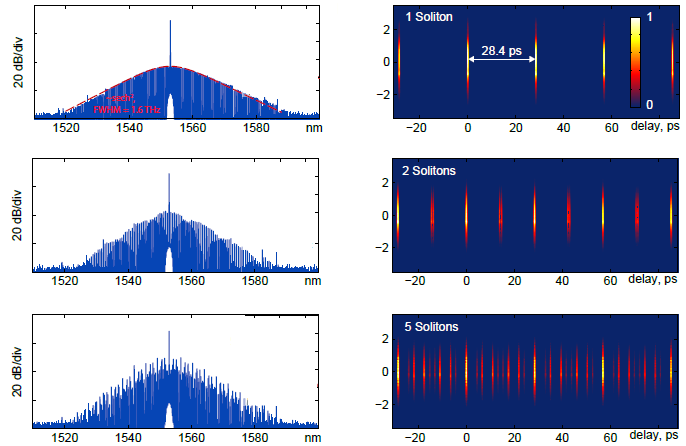
\includegraphics[]{experiment}
  \caption{Экспериментально полученный спектр гребенки для одно, двух и пяти солитонного режимов. Справа картина импульсов во временном представлении. Взято из \cite{mlg_to_nature}} \label{experiment}
\end{figure}

Обзор потенциальных применений оптических гребенок в микрорезонаторах дан в \cite{ScienceMag}. Используя компактные микрорезонаторы и один лазер накачки, можно сделать калибровку для астрономического спектрографа для видимого и ближнего ИК диапазонов, с межмодовым расстоянием $10-30$ ГГц. Такие устройства могут позволить измерить доплеровский сдвиг в спектре звезды с точностью, требуемой для обнаружения планет вне Солнечной системы. Ключевым преимуществом в этом случае является малый размер и масса системы.

Гребенки в микрорезонаторах могут использоваться в прямой спектроскопии атомов и молекул по тем же методам, что были разработаны для оптических гребенок с использованием фемтосекундного лазера (по Т. Хэншу). В установке используются две гребенки (которые могут располагаться на одном чипе), имеющие немного различные межмодовые интервалы. Одна гребенка используется как локальный осциллятор, другая используются для получения оптической спектральной картины исследуемого образца. Результирующие биения двух гребенок дают радиочастотный сигнал, содержащий информацию о линиях поглощения.

Генерация оптических гребенок с высокой мощностью на каждую линию ($>1$ мВт) и межмодовым интервалом в $10,25,50,100$ ГГц может использоваться в многоканальной оптической телекоммуникации на частотах $1450-1750$ нм. Микрорезонатор и один мощный лазер может заменить индивидуальные лазеры для каждого телекоммуникационного канала.

В работе \cite{coherent_data_transmission} экспериментально продемонстрировано использование оптических гребенок в микрорезонаторе в роли оптического источника в установке для спектрального уплотнения телекоммуникационных каналов и когерентной передачи данных с использованием амплитудно и фазово модулированных несущих. Достигнута пропускная способность $392$ Гбит/с.

Другим применением могут быть оптические часы. Экспериментальная демонстрация таких часов дана в \cite{frequency_comb_optical_clock}. Модулированный по амплитуде лазер с максимальной мощностью $140$ мВт возбуждает кольцевой резонатор из плавленного кварца (расположен на чипе, добротность $Q=6\times10^7$). Генерируется гребенка, покрывающая $20$ нм интервал около накачки $1560$ нм. Межмодовое расстояние составило $33$ ГГц. Далее гребенка расширяется до $200$ нм при ее пропускании через сильно нелинейное волокно. Новый спектр покрывает частоту рубидиевого стандарта (после удвоения частоты). Выбираются две линии гребенки на расстояний 108 мод друг от друга ($1560$ и $1590$ нм соответственно), которые привязываются через дополнительные лазеры к рубидиевым переходам. Выходным сигналом часов является разность частот этих двух стабилизированных лазеров. Она составила $32.9819213$ ГГц. Девиация Аллана достигала $5\times10^{-11}$ при измерении за $10^4$ сек.

В работах \cite{MLG_nature_2012}, \cite{mw_signals_generation} продемонстрирована возможность генерации СВЧ сигналов с малым шумом, используя оптические частотные гребенки. Частота СВЧ сигнала определяется межмодовым интервалом гребенки.
%Установка \cite{mlg_to_nature} для наблюдения оптических гребенок (рис. \ref{scheme}) состоит из лазера с узкой линией, работающего в непрерывном режиме генерации, используемого для накачки микрорезонатора из нелинейного материала. Связь с резонатором происходит через срезанное под острым углом или растянутое волокно, призму. Гребенки наблюдаются с помощью анализатора спектра. Используется резонаторы в форме тороида, сферы или диска \cite{ScienceMag}. Гребенки наблюдались для резонаторов с добротностью $10^7-10^9$ \cite{MLG_nature_2012} и для резонаторов в интегральном исполнении с добротностью $10^6$.



